\ProvidesFile{seminar05.tex}

\section{Семинар 5}

\subsection{Задача 1}

Докажите, что любая нетождественная перестановка единственным образом представима в виде произведения независимых циклов.

\begin{proof}

Рассмотрим элемент 1. Он переходит в $\sigma(1)$ под действием перестановки $\sigma$.

Если 1 перешла в себя, то цикл закончился.

Если 1 перешла не в себя, то рассматриваем $\sigma(\sigma(1)), \ldots \sigma^k(1)$. Рано или поздно мы перейдем в единицу.

В любом случае, мы получили какой-то цикл. Запомним его.

Рассмотрим $i$, который не участвовал в этом цикле и проделаем с ним то же самое. Получим ещё один цикл. Продолжаем так действовать до тех пор, пока все элементы не распадутся в циклы. Это обеспечивает существование такого произведения независимых циклов.

Ясно, что каждый элемент присутствует только в одном цикле (то есть зная лишь один элемент цикла, мы понимаем, как устроен весь цикл). Это обеспечивает единственность (с точностью до перестановки циклов).
\end{proof}

\subsection{Задача 2}

Докажите, что любая перестановка $\sigma$ в некоторой степени дает тождественную перестановку $id$.

\begin{proof}
Если $\sigma = id$, то и доказывать нечего.

Если $\sigma \neq id$, то давайте рассмотрим представление этой перестановки в виде произведения независимых циклов. Возьмём произведение длин этих циклов и победим.
\end{proof}

\subsection{Задача 3}

Докажите, что порядок перестановки равен наименьшему общему кратному длин
независимых циклов, в произведение которых раскладывается перестановка.

\begin{proof}
Если $\sigma = id$, то и доказывать нечего.

Если $\sigma \neq id$, то давайте рассмотрим представление этой перестановки в виде произведения независимых циклов. Ясно, что каждый из циклов возвращает действует на своих элементов тождественно тогда и только тогда, когда он применен $k \cdot \alpha_i$ раз, где $\alpha_i$ - длина соответствующего независимого цикла, $k$ - натуральное.

Значит, порядок перестановки должен делить длину каждого независимого цикла. Вот и получается, что порядок перестановки хотя бы НОК.

Предположим, что мы нашли число $q$, меньшее НОКа, для которого $\sigma^q = id$. $q$ делится на длину каждого цикла. Но тогда и получается, что $q$ хотя бы НОК.
\end{proof}

\subsection{Задача 4}
Илья взял собранный кубик Рубика, проделал над ним некоторую комбинацию вращений и положил на место. Докажите, что можно повторить точно такие же действия
над кубиком еще несколько раз, чтобы он оказался вновь в собранном состоянии.

\begin{proof}

Илья действует перестановками $\sigma_1, \sigma_2, \ldots, \sigma_n$ на кубике Рубика. Если Илья в результате $\sigma_n \cdot \ldots \sigma_1$ привёл кубик Рубика в собранное состояние, то и доказывать нечего.

Иначе давайте применять эти перестановки так, что в какой-то момент две из них повторяться (кубик Рубика имеет конечное число состояний, значит, точно повторится) $\sigma_1 \cdot \ldots \sigma_i = \sigma_1 \cdot \ldots \sigma_j$. Пусть справа множителей больше. Домножим обе части на $(\sigma_{i+1} \cdot \ldots \cdot \sigma_j)^-1$ (то есть просто откатимся на несколько действий). И тогда получим: $\sigma_1 \cdot \ldots \sigma_i = id$

\end{proof}

\subsection{Задача 5}

Любая транспозиция является нечетной перестановкой

\begin{definition}
\label{claim::ElementaryTransposition}
Элементарная транспозиция - транспозиция элементов $i, i+1$.
\end{definition}

\begin{claim*}
Элементарная транспозиция меняет знак перестановки (то есть количество инверсий на 1).
\end{claim*}

\begin{proof}
Ну действительно: если элементарная транспозиция меняет местами два элемента подряд, то было так, что $i < i+1$, а после перестановки они поменялись местами. Вот и получилась смена знака.

Далее заметим, что любая транспозиция  распадается в $2k - 1$ элементарную транспозицию. Действительно: нужно $k$ свапов, чтобы $i$-ый элемнт встал в $j$-ую ячейку. После этого нужно $k - 1$ свапов, чтобы $j$-ый элемент в стал в $i$-ую ячейку. Но $2k - 1$ это нечетное число, каждая элементарная транспозиция меняет знак, поэтому поменяется знак $2k - 1$ раз, то есть нечетное число раз.
\end{proof}

\begin{figure}[h]
    \centering
    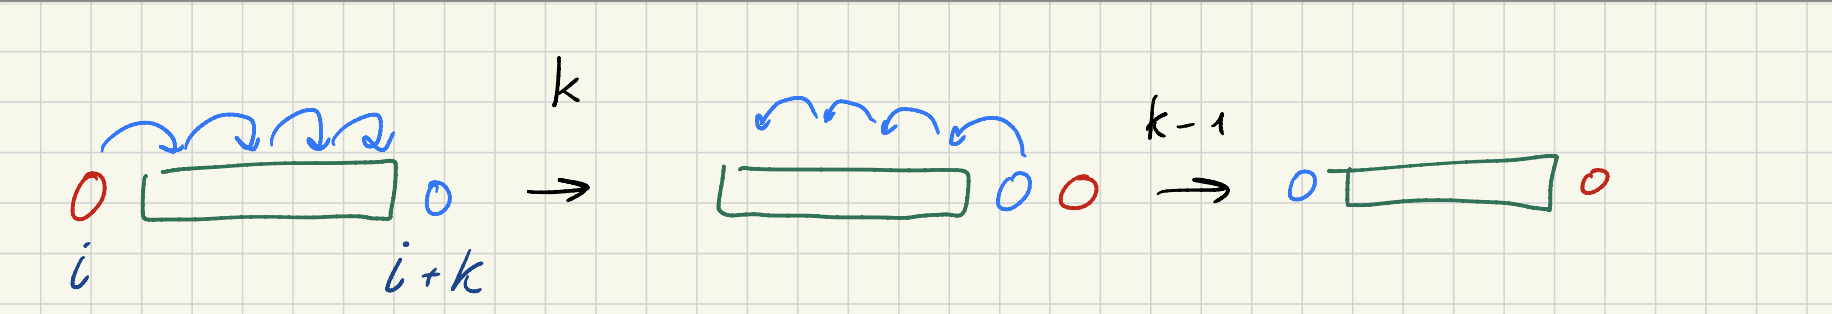
\includegraphics[width=1\linewidth]{Figures/sem5_task7.png}
\end{figure}

\subsection{Задача 6}
Домножение любой перестановки на транспозицию меняет четность исходной перестановки.
\begin{proof}
Каждая транспозиция распадается в $2k - 1$ элементарных (по 5-ой задаче), и каждая элементарная транспозиция меняет знак. Получается, транспозиция меняет знак.
\end{proof}

\subsection{Задача 7}

\begin{enumerate}[label=\asbuk*)]
\item Любая перестановка представима в виде произведения нескольких транспозиций.
\item Та же задача) На уроке физкультуры школьники некоторого класса выстроились
в шеренгу. Учитель может попросить любых двух школьников поменяться местами.
Докажите, что он всегда может расставить школьников по росту.
\end{enumerate}

\begin{proof}
Оба пункта решаются идей пузырьковой сортировки. По сути на это можно смотреть так: применение элементарной транспозиции -- это просто swap двух элементов. Последовательно поднимаем <<пузырьком>> элементы так, чтобы все стояли на своих местах.
\end{proof}

\subsection{Задача 8}
Цикл длины $k$ является четной перестановкой тогда и только тогда, когда $k$ нечетно.

\begin{proof}
Любой цикл длины $k$ распадается в $k-1$ транспозицию. Применение $k-1$ транспозиции меняет знак $k-1$ раз. Вот и получается, что цикл длины $k$ является четным тогда и только тогда, когда $k$ нечетно.
\end{proof}

\subsection{Задача 9}

При умножении любой перестановки на четную перестановку четность исходной перестановки сохраняется, при умножении на нечетную перестановку четность меняется.

Оставлю доказательство Димы.

\begin{claim*}
Пусть $\sigma,\tau\in\Sym{n}$ -- произвольные перестановки, тогда 
\[
\sgn(\sigma\tau) = \sgn(\sigma)\sgn(\tau)\quad
\]
\end{claim*}
\begin{proof}
Надо показать, что
\[
d(\sigma) + d(\tau) = d(\sigma \tau) \pmod 2
\]
Давайте фиксируем пару $i, j$ и докажем следующее равенство
\[
d_{ij}(\tau) + d_{\tau(i)\tau(j)}(\sigma) = d_{ij}(\sigma \tau) \pmod 2
\]
Возможны следующие $4$ случая:
\begin{align*}
&{
\begin{matrix}
{\tau}\\{}\\{\sigma}
\end{matrix}\quad
\begin{aligned}
\xymatrix@R=10pt@C=10pt{
	{i}\ar[dr]&{}&{j}\ar[dr]&{}\\
	{}&{\tau(i)}\ar[d]&{}&{\tau(j)}\ar[dl]\\
	{}&{\sigma\tau(i)}&{\sigma\tau(j)}&{}\\
}
\end{aligned}
}&&{
\begin{matrix}
{\tau}\\{}\\{\sigma}
\end{matrix}\quad
\begin{aligned}
\xymatrix@R=10pt@C=10pt{
	{i}\ar[drrr]&{}&{j}\ar[dl]&{}\\
	{}&{\tau(j)}\ar[d]&{}&{\tau(i)}\ar[dl]\\
	{}&{\sigma\tau(j)}&{\sigma\tau(i)}&{}\\
}
\end{aligned}
}\\
&{
\begin{matrix}
{\tau}\\{}\\{\sigma}
\end{matrix}\quad
\begin{aligned}
\xymatrix@R=10pt@C=10pt{
	{i}\ar[dr]&{}&{j}\ar[dr]&{}\\
	{}&{\tau(i)}\ar[dr]&{}&{\tau(j)}\ar[dll]\\
	{}&{\sigma\tau(j)}&{\sigma\tau(i)}&{}\\
}
\end{aligned}
}&&{
\begin{matrix}
{\tau}\\{}\\{\sigma}
\end{matrix}\quad
\begin{aligned}
\xymatrix@R=10pt@C=10pt{
	{i}\ar[drrr]&{}&{j}\ar[dl]&{}\\
	{}&{\tau(j)}\ar[dr]&{}&{\tau(i)}\ar[dll]\\
	{}&{\sigma\tau(i)}&{\sigma\tau(j)}&{}\\
}
\end{aligned}
}\\
\end{align*}
Занесем результаты в таблицу
\begin{center}
\begin{tabular}{|c|c|c|c|c|}
\hline
{$d_{ij}(\tau)$}&{0}&{1}&{0}&{1}\\
\hline
{$d_{\tau(i)\tau(j)}(\sigma)$}&{0}&{0}&{1}&{1}\\
\hline
{$d_{ij} + d_{\tau(i)\tau(j)}(\sigma)$}&{0}&{1}&{1}&{2}\\
\hline
{$d_{ij}(\sigma\tau)$}&{0}&{1}&{1}&{0}\\
\hline
\end{tabular}
\end{center}
Что доказывает равенство
\[
d_{ij}(\tau) + d_{\tau(i)\tau(j)}(\sigma) = d_{ij}(\sigma \tau) \pmod 2
\]
Теперь сложим его для всех пар $i < j$.
Получим
\[
\sum_{i<j}d_{ij}(\tau) + \sum_{i<j}d_{\tau(i)\tau(j)}(\sigma) = \sum_{i<j}d_{ij}(\sigma \tau) \pmod 2
\]
Откуда
\[
d(\tau) + \sum_{i<j}d_{\tau(i)\tau(j)}(\sigma) = d(\sigma \tau) \pmod 2
\]
Так как $\tau\colon X_n\to X_n$ -- биекция, то если $(i,j)$ пробегает все разные пары, то и $(\tau(i),\tau(j))$ пробегает все разные пары.
Значит оставшаяся сумма равна $d(\sigma)$, что завершает доказательство.
\end{proof}

\subsection{Задача 10}
Четных перестановок $n$ элементов столько же, сколько и нечетных, то есть и тех, и других ровно $\frac{n!}{2}$.

\begin{proof}
Нужно лишь показать, что между четными и нечетными перестановками есть биекция. Но это совсем просто сделать. Из любой четной перестановки при помощи транспозиции (1; 2) можно получить нечетную, а из получившейся нечетной с помощью этой же транспозиции можно получить исходную чётную.

Значит, эта биекция и в правду есть, но тогда количество четных и нечетных перестановок равны. Всего перестановок $n!$, тогда четных и нечетных по $\frac{n!}{2}$
\end{proof}

\subsection{Задача 11}

\textbf{Игра в пятнашки.} В таблицу $4 \times 4$ вписаны подряд (слева направо, сверху вниз) числа от 1 до 15, так, что правый нижний угол остался свободным. За ход можно сдвинуть
на свободное место любое из чисел, которое соседствует с ним по стороне (и таким
образом свободное место поменяет свое расположение). Докажите, что такими ходами нельзя получить комбинацию, отличающуюся от исходной лишь транспозицией
чисел 14 и 15.

\begin{proof}
Давайте назовём пустое место числом 0.

Тогда нам разрешены лишь <<элементарные>> транспозиции с нулём. <<Элементарные>> в том плане, что мы можем их свапнуть в этой игре лишь с теми числами, которые стоят с нулём, а не в смысле определения \ref{claim::ElementaryTransposition}. Ну вообще формально говоря, нехорошо делать перестановку на множестве с нулем, так как перестановка бьёт из множества $\{1, ..., n\}$ в себя, но очевидно, что между ними есть биекция, поэтому пофиг.

Пусть мы смогли с помощью перестановки $\sigma$ (не обязательно той, что является композицией элементарных транспозиций) добиться того, что 14 и 15 поменялись местами. Тогда мы подействовали транспозицией 14 и 15. А транспозиция это вообще говоря нечетная перестановка. Значит, если за $N$ ходов мы сможем добиться того, что 14 и 15 поменялись местами, то $N$ обязательно нечетно. 

С другой стороны, нам разрешены только <<элементарные>> преобразования с нулём, поэтому каждое действие - это применение транспозиции с нулём. За одно действие ноль двигается в одно из четырёх направлений: влево, вправо, вниз, вверх. В результате наших преобразований ноль вернулся на то же место. Значит, число преобразований влево было таким же, как и число преобразований вправо и аналогично по вертикали. В итоге получаем, что на самом деле наша перестановка является четной. Но так как каждая транспозиция нечетна, то $N$ -- четно. Получили противоречие с тем, что $N$ -- нечетно.
\end{proof}